\documentclass[twoside]{book}

% Packages required by doxygen
\usepackage{fixltx2e}
\usepackage{calc}
\usepackage{doxygen}
\usepackage[export]{adjustbox} % also loads graphicx
\usepackage{graphicx}
\usepackage[utf8]{inputenc}
\usepackage{makeidx}
\usepackage{multicol}
\usepackage{multirow}
\PassOptionsToPackage{warn}{textcomp}
\usepackage{textcomp}
\usepackage[nointegrals]{wasysym}
\usepackage[table]{xcolor}

% Font selection
\usepackage[T1]{fontenc}
\usepackage[scaled=.90]{helvet}
\usepackage{courier}
\usepackage{amssymb}
\usepackage{sectsty}
\renewcommand{\familydefault}{\sfdefault}
\allsectionsfont{%
  \fontseries{bc}\selectfont%
  \color{darkgray}%
}
\renewcommand{\DoxyLabelFont}{%
  \fontseries{bc}\selectfont%
  \color{darkgray}%
}
\newcommand{\+}{\discretionary{\mbox{\scriptsize$\hookleftarrow$}}{}{}}

% Page & text layout
\usepackage{geometry}
\geometry{%
  a4paper,%
  top=2.5cm,%
  bottom=2.5cm,%
  left=2.5cm,%
  right=2.5cm%
}
\tolerance=750
\hfuzz=15pt
\hbadness=750
\setlength{\emergencystretch}{15pt}
\setlength{\parindent}{0cm}
\setlength{\parskip}{3ex plus 2ex minus 2ex}
\makeatletter
\renewcommand{\paragraph}{%
  \@startsection{paragraph}{4}{0ex}{-1.0ex}{1.0ex}{%
    \normalfont\normalsize\bfseries\SS@parafont%
  }%
}
\renewcommand{\subparagraph}{%
  \@startsection{subparagraph}{5}{0ex}{-1.0ex}{1.0ex}{%
    \normalfont\normalsize\bfseries\SS@subparafont%
  }%
}
\makeatother

% Headers & footers
\usepackage{fancyhdr}
\pagestyle{fancyplain}
\fancyhead[LE]{\fancyplain{}{\bfseries\thepage}}
\fancyhead[CE]{\fancyplain{}{}}
\fancyhead[RE]{\fancyplain{}{\bfseries\leftmark}}
\fancyhead[LO]{\fancyplain{}{\bfseries\rightmark}}
\fancyhead[CO]{\fancyplain{}{}}
\fancyhead[RO]{\fancyplain{}{\bfseries\thepage}}
\fancyfoot[LE]{\fancyplain{}{}}
\fancyfoot[CE]{\fancyplain{}{}}
\fancyfoot[RE]{\fancyplain{}{\bfseries\scriptsize Generated by Doxygen }}
\fancyfoot[LO]{\fancyplain{}{\bfseries\scriptsize Generated by Doxygen }}
\fancyfoot[CO]{\fancyplain{}{}}
\fancyfoot[RO]{\fancyplain{}{}}
\renewcommand{\footrulewidth}{0.4pt}
\renewcommand{\chaptermark}[1]{%
  \markboth{#1}{}%
}
\renewcommand{\sectionmark}[1]{%
  \markright{\thesection\ #1}%
}

% Indices & bibliography
\usepackage{natbib}
\usepackage[titles]{tocloft}
\setcounter{tocdepth}{3}
\setcounter{secnumdepth}{5}
\makeindex

% Hyperlinks (required, but should be loaded last)
\usepackage{ifpdf}
\ifpdf
  \usepackage[pdftex,pagebackref=true]{hyperref}
\else
  \usepackage[ps2pdf,pagebackref=true]{hyperref}
\fi
\hypersetup{%
  colorlinks=true,%
  linkcolor=blue,%
  citecolor=blue,%
  unicode%
}

% Custom commands
\newcommand{\clearemptydoublepage}{%
  \newpage{\pagestyle{empty}\cleardoublepage}%
}

\usepackage{caption}
\captionsetup{labelsep=space,justification=centering,font={bf},singlelinecheck=off,skip=4pt,position=top}

%===== C O N T E N T S =====

\begin{document}

% Titlepage & ToC
\hypersetup{pageanchor=false,
             bookmarksnumbered=true,
             pdfencoding=unicode
            }
\pagenumbering{roman}
\begin{titlepage}
\vspace*{7cm}
\begin{center}%
{\Large My Project }\\
\vspace*{1cm}
{\large Generated by Doxygen 1.8.11}\\
\end{center}
\end{titlepage}
\clearemptydoublepage
\tableofcontents
\clearemptydoublepage
\pagenumbering{arabic}
\hypersetup{pageanchor=true}

%--- Begin generated contents ---
\chapter{File Index}
\section{File List}
Here is a list of all files with brief descriptions\+:\begin{DoxyCompactList}
\item\contentsline{section}{\hyperlink{Lab1_8c}{Lab1.\+c} }{\pageref{Lab1_8c}}{}
\end{DoxyCompactList}

\chapter{File Documentation}
\hypertarget{BoothMultAlg_8cpp}{}\section{Booth\+Mult\+Alg.\+cpp File Reference}
\label{BoothMultAlg_8cpp}\index{Booth\+Mult\+Alg.\+cpp@{Booth\+Mult\+Alg.\+cpp}}
{\ttfamily \#include $<$iostream$>$}\\*
{\ttfamily \#include $<$conio.\+h$>$}\\*
Include dependency graph for Booth\+Mult\+Alg.\+cpp\+:
\nopagebreak
\begin{figure}[H]
\begin{center}
\leavevmode
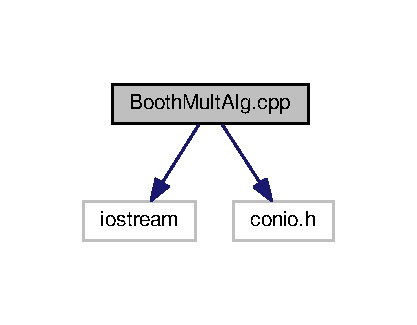
\includegraphics[width=200pt]{BoothMultAlg_8cpp__incl}
\end{center}
\end{figure}
\subsection*{Functions}
\begin{DoxyCompactItemize}
\item 
void \hyperlink{BoothMultAlg_8cpp_a28d175fae0a95b0469371584e359a794}{add} (int a\mbox{[}$\,$\mbox{]}, int x\mbox{[}$\,$\mbox{]}, int qrn)
\item 
void \hyperlink{BoothMultAlg_8cpp_a2d62bc1d3b84866aad12f9047e2335f6}{complement} (int a\mbox{[}$\,$\mbox{]}, int n)
\item 
void \hyperlink{BoothMultAlg_8cpp_ab48116c2ea057272ced3e4c25de5e1ec}{ashr} (int ac\mbox{[}$\,$\mbox{]}, int qr\mbox{[}$\,$\mbox{]}, int \&qn, int qrn)
\item 
void \hyperlink{BoothMultAlg_8cpp_a25f0bd412c1524aaaf3d3e573038d367}{display} (int ac\mbox{[}$\,$\mbox{]}, int qr\mbox{[}$\,$\mbox{]}, int qrn)
\item 
int \hyperlink{BoothMultAlg_8cpp_a3c04138a5bfe5d72780bb7e82a18e627}{main} (int argc, char $\ast$$\ast$argv)
\end{DoxyCompactItemize}


\subsection{Function Documentation}
\index{Booth\+Mult\+Alg.\+cpp@{Booth\+Mult\+Alg.\+cpp}!add@{add}}
\index{add@{add}!Booth\+Mult\+Alg.\+cpp@{Booth\+Mult\+Alg.\+cpp}}
\subsubsection[{\texorpdfstring{add(int a[], int x[], int qrn)}{add(int a[], int x[], int qrn)}}]{\setlength{\rightskip}{0pt plus 5cm}void add (
\begin{DoxyParamCaption}
\item[{int}]{a\mbox{[}$\,$\mbox{]}, }
\item[{int}]{x\mbox{[}$\,$\mbox{]}, }
\item[{int}]{qrn}
\end{DoxyParamCaption}
)}\hypertarget{BoothMultAlg_8cpp_a28d175fae0a95b0469371584e359a794}{}\label{BoothMultAlg_8cpp_a28d175fae0a95b0469371584e359a794}

\begin{DoxyCode}
21 \{
22     \textcolor{keywordtype}{int} i, c = 0;
23     \textcolor{keywordflow}{for} (i = 0; i < qrn; i++)
24     \{
25         ac[i] = ac[i] + x[i] + c;
26         \textcolor{keywordflow}{if} (ac[i] > 1)
27         \{
28             ac[i] = ac[i] % 2;
29             c = 1;
30         \}
31         \textcolor{keywordflow}{else}
32             c = 0;
33     \}
34  
35 \}
\end{DoxyCode}
\index{Booth\+Mult\+Alg.\+cpp@{Booth\+Mult\+Alg.\+cpp}!ashr@{ashr}}
\index{ashr@{ashr}!Booth\+Mult\+Alg.\+cpp@{Booth\+Mult\+Alg.\+cpp}}
\subsubsection[{\texorpdfstring{ashr(int ac[], int qr[], int \&qn, int qrn)}{ashr(int ac[], int qr[], int &qn, int qrn)}}]{\setlength{\rightskip}{0pt plus 5cm}void ashr (
\begin{DoxyParamCaption}
\item[{int}]{ac\mbox{[}$\,$\mbox{]}, }
\item[{int}]{qr\mbox{[}$\,$\mbox{]}, }
\item[{int \&}]{qn, }
\item[{int}]{qrn}
\end{DoxyParamCaption}
)}\hypertarget{BoothMultAlg_8cpp_ab48116c2ea057272ced3e4c25de5e1ec}{}\label{BoothMultAlg_8cpp_ab48116c2ea057272ced3e4c25de5e1ec}

\begin{DoxyCode}
38 \{
39     \textcolor{keywordtype}{int} temp, i;
40  
41     temp = ac[0];
42     qn = qr[0];
43     cout << \textcolor{stringliteral}{"\(\backslash\)t\(\backslash\)tashr\(\backslash\)t\(\backslash\)t"};
44     \textcolor{keywordflow}{for} (i = 0; i < qrn - 1; i++)
45     \{
46         ac[i] = ac[i + 1];
47         qr[i] = qr[i + 1];
48     \}
49     qr[qrn - 1] = temp;
50 \}
\end{DoxyCode}
\index{Booth\+Mult\+Alg.\+cpp@{Booth\+Mult\+Alg.\+cpp}!complement@{complement}}
\index{complement@{complement}!Booth\+Mult\+Alg.\+cpp@{Booth\+Mult\+Alg.\+cpp}}
\subsubsection[{\texorpdfstring{complement(int a[], int n)}{complement(int a[], int n)}}]{\setlength{\rightskip}{0pt plus 5cm}void complement (
\begin{DoxyParamCaption}
\item[{int}]{a\mbox{[}$\,$\mbox{]}, }
\item[{int}]{n}
\end{DoxyParamCaption}
)}\hypertarget{BoothMultAlg_8cpp_a2d62bc1d3b84866aad12f9047e2335f6}{}\label{BoothMultAlg_8cpp_a2d62bc1d3b84866aad12f9047e2335f6}

\begin{DoxyCode}
8 \{
9     \textcolor{keywordtype}{int} i;
10  
11     \textcolor{keywordtype}{int} x[8] = \{ NULL \};
12     x[0] = 1;
13     \textcolor{keywordflow}{for} (i = 0; i < n; i++)
14     \{
15         a[i] = (a[i] + 1) % 2;
16     \}
17     \hyperlink{BoothMultAlg_8cpp_a28d175fae0a95b0469371584e359a794}{add}(a, x, n);
18 \}
\end{DoxyCode}


Here is the call graph for this function\+:
\nopagebreak
\begin{figure}[H]
\begin{center}
\leavevmode
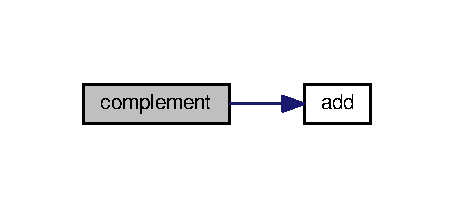
\includegraphics[width=218pt]{BoothMultAlg_8cpp_a2d62bc1d3b84866aad12f9047e2335f6_cgraph}
\end{center}
\end{figure}


\index{Booth\+Mult\+Alg.\+cpp@{Booth\+Mult\+Alg.\+cpp}!display@{display}}
\index{display@{display}!Booth\+Mult\+Alg.\+cpp@{Booth\+Mult\+Alg.\+cpp}}
\subsubsection[{\texorpdfstring{display(int ac[], int qr[], int qrn)}{display(int ac[], int qr[], int qrn)}}]{\setlength{\rightskip}{0pt plus 5cm}void display (
\begin{DoxyParamCaption}
\item[{int}]{ac\mbox{[}$\,$\mbox{]}, }
\item[{int}]{qr\mbox{[}$\,$\mbox{]}, }
\item[{int}]{qrn}
\end{DoxyParamCaption}
)}\hypertarget{BoothMultAlg_8cpp_a25f0bd412c1524aaaf3d3e573038d367}{}\label{BoothMultAlg_8cpp_a25f0bd412c1524aaaf3d3e573038d367}

\begin{DoxyCode}
53 \{
54     \textcolor{keywordtype}{int} i;
55  
56     \textcolor{keywordflow}{for} (i = qrn - 1; i >= 0; i--)
57         cout << ac[i];
58     cout << \textcolor{stringliteral}{" "};
59     \textcolor{keywordflow}{for} (i = qrn - 1; i >= 0; i--)
60         cout << qr[i];
61  
62 \}
\end{DoxyCode}
\index{Booth\+Mult\+Alg.\+cpp@{Booth\+Mult\+Alg.\+cpp}!main@{main}}
\index{main@{main}!Booth\+Mult\+Alg.\+cpp@{Booth\+Mult\+Alg.\+cpp}}
\subsubsection[{\texorpdfstring{main(int argc, char $\ast$$\ast$argv)}{main(int argc, char **argv)}}]{\setlength{\rightskip}{0pt plus 5cm}int main (
\begin{DoxyParamCaption}
\item[{int}]{argc, }
\item[{char $\ast$$\ast$}]{argv}
\end{DoxyParamCaption}
)}\hypertarget{BoothMultAlg_8cpp_a3c04138a5bfe5d72780bb7e82a18e627}{}\label{BoothMultAlg_8cpp_a3c04138a5bfe5d72780bb7e82a18e627}

\begin{DoxyCode}
65 \{
66     \textcolor{keywordtype}{int} mt[10], br[10], qr[10], sc, ac[10] = \{ 0 \};
67     \textcolor{keywordtype}{int} brn, qrn, i, qn, temp;
68     cout
69             << \textcolor{stringliteral}{"\(\backslash\)n--Enter the multiplicand and multipier in signed 2's complement form if negative--"};
70  
71     cout << \textcolor{stringliteral}{"\(\backslash\)n Number of multiplicand bit="};
72     cin >> brn;
73     cout << \textcolor{stringliteral}{"\(\backslash\)nmultiplicand="};
74  
75     \textcolor{keywordflow}{for} (i = brn - 1; i >= 0; i--)
76         cin >> br[i]; \textcolor{comment}{//multiplicand}
77  
78     \textcolor{keywordflow}{for} (i = brn - 1; i >= 0; i--)
79         mt[i] = br[i]; \textcolor{comment}{// copy multipier to temp array mt[]}
80  
81     \hyperlink{BoothMultAlg_8cpp_a2d62bc1d3b84866aad12f9047e2335f6}{complement}(mt, brn);
82  
83     cout << \textcolor{stringliteral}{"\(\backslash\)nNo. of multiplier bit="};
84     cin >> qrn;
85  
86     sc = qrn; \textcolor{comment}{//sequence counter}
87  
88     cout << \textcolor{stringliteral}{"Multiplier="};
89     \textcolor{keywordflow}{for} (i = qrn - 1; i >= 0; i--)
90         cin >> qr[i]; \textcolor{comment}{//multiplier}
91  
92  
93     qn = 0;
94     temp = 0;
95  
96     cout << \textcolor{stringliteral}{"qn\(\backslash\)tq[n+1]\(\backslash\)t\(\backslash\)tBR\(\backslash\)t\(\backslash\)tAC\(\backslash\)tQR\(\backslash\)t\(\backslash\)tsc\(\backslash\)n"};
97     cout << \textcolor{stringliteral}{"\(\backslash\)t\(\backslash\)t\(\backslash\)tinitial\(\backslash\)t\(\backslash\)t"};
98     \hyperlink{BoothMultAlg_8cpp_a25f0bd412c1524aaaf3d3e573038d367}{display}(ac, qr, qrn);
99     cout << \textcolor{stringliteral}{"\(\backslash\)t\(\backslash\)t"} << sc << \textcolor{stringliteral}{"\(\backslash\)n"};
100  
101     \textcolor{keywordflow}{while} (sc != 0)
102     \{
103         cout << qr[0] << \textcolor{stringliteral}{"\(\backslash\)t"} << qn;
104         \textcolor{keywordflow}{if} ((qn + qr[0]) == 1)
105         \{
106             \textcolor{keywordflow}{if} (temp == 0)
107             \{
108                 \hyperlink{BoothMultAlg_8cpp_a28d175fae0a95b0469371584e359a794}{add}(ac, mt, qrn);
109                 cout << \textcolor{stringliteral}{"\(\backslash\)t\(\backslash\)tsubtracting BR\(\backslash\)t"};
110                 \textcolor{keywordflow}{for} (i = qrn - 1; i >= 0; i--)
111                     cout << ac[i];
112                 temp = 1;
113             \}
114             \textcolor{keywordflow}{else} \textcolor{keywordflow}{if} (temp == 1)
115             \{
116                 \hyperlink{BoothMultAlg_8cpp_a28d175fae0a95b0469371584e359a794}{add}(ac, br, qrn);
117                 cout << \textcolor{stringliteral}{"\(\backslash\)t\(\backslash\)tadding BR\(\backslash\)t"};
118                 \textcolor{keywordflow}{for} (i = qrn - 1; i >= 0; i--)
119                     cout << ac[i];
120                 temp = 0;
121             \}
122             cout << \textcolor{stringliteral}{"\(\backslash\)n\(\backslash\)t"};
123             \hyperlink{BoothMultAlg_8cpp_ab48116c2ea057272ced3e4c25de5e1ec}{ashr}(ac, qr, qn, qrn);
124         \}
125         \textcolor{keywordflow}{else} \textcolor{keywordflow}{if} (qn - qr[0] == 0)
126             \hyperlink{BoothMultAlg_8cpp_ab48116c2ea057272ced3e4c25de5e1ec}{ashr}(ac, qr, qn, qrn);
127  
128         \hyperlink{BoothMultAlg_8cpp_a25f0bd412c1524aaaf3d3e573038d367}{display}(ac, qr, qrn);
129         cout << \textcolor{stringliteral}{"\(\backslash\)t"};
130  
131         sc--;
132         cout << \textcolor{stringliteral}{"\(\backslash\)t"} << sc << \textcolor{stringliteral}{"\(\backslash\)n"};
133     \}
134     cout << \textcolor{stringliteral}{"Result="};
135     \hyperlink{BoothMultAlg_8cpp_a25f0bd412c1524aaaf3d3e573038d367}{display}(ac, qr, qrn);
136 \}\end{DoxyCode}


Here is the call graph for this function\+:
\nopagebreak
\begin{figure}[H]
\begin{center}
\leavevmode
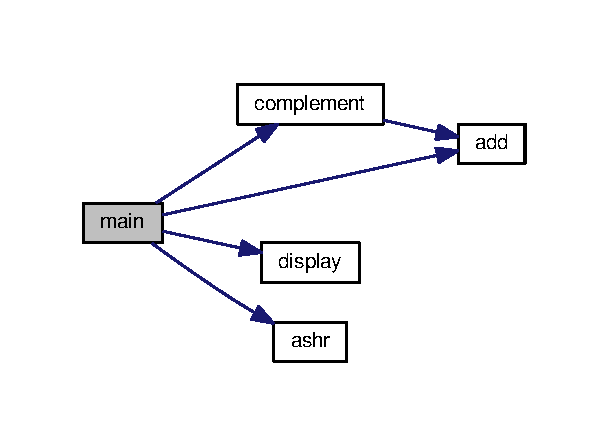
\includegraphics[width=292pt]{BoothMultAlg_8cpp_a3c04138a5bfe5d72780bb7e82a18e627_cgraph}
\end{center}
\end{figure}



%--- End generated contents ---

% Index
\backmatter
\newpage
\phantomsection
\clearemptydoublepage
\addcontentsline{toc}{chapter}{Index}
\printindex

\end{document}
